\begin{knitrout}
\definecolor{shadecolor}{rgb}{1, 1, 1}\color{fgcolor}\begin{kframe}
\begin{alltt}
\hlkwd{library}\hlstd{(np)}

\hlstd{x.eval} \hlkwb{<-} \hlkwd{seq}\hlstd{(}\hlopt{-}\hlnum{0.2}\hlstd{,} \hlnum{0.2}\hlstd{,} \hlkwc{length.out} \hlstd{=} \hlnum{200}\hlstd{)}

\hlstd{h_normal_np} \hlkwb{<-} \hlkwd{npudensbw}\hlstd{(}\hlkwc{dat} \hlstd{= x,} \hlkwc{bwmethod} \hlstd{=} \hlstr{"normal-reference"}\hlstd{)}

\hlstd{dens.ksum} \hlkwb{<-} \hlkwd{npksum}\hlstd{(}
 \hlkwc{txdat} \hlstd{= x,}
 \hlkwc{exdat} \hlstd{= x.eval,}
 \hlkwc{bws} \hlstd{= h_normal_np}\hlopt{$}\hlstd{bw}
\hlstd{)}\hlopt{$}\hlstd{ksum} \hlopt{/} \hlstd{(n} \hlopt{*} \hlstd{h_normal_np}\hlopt{$}\hlstd{bw[}\hlnum{1}\hlstd{])}

\hlstd{dens.ksum.df} \hlkwb{<-} \hlkwd{data.frame}\hlstd{(}\hlkwc{x} \hlstd{= x.eval,} \hlkwc{y} \hlstd{= dens.ksum)}

\hlkwd{ggplot}\hlstd{(x_df,} \hlkwd{aes}\hlstd{(x))} \hlopt{+}
 \hlkwd{geom_histogram}\hlstd{(}
   \hlkwd{aes}\hlstd{(}\hlkwc{y} \hlstd{= ..density..),}
   \hlkwc{binwidth} \hlstd{= h_normal_np}\hlopt{$}\hlstd{bw,}
   \hlkwc{col} \hlstd{=} \hlstr{"black"}\hlstd{,}
   \hlkwc{fill} \hlstd{=} \hlstr{"white"}
 \hlstd{)} \hlopt{+}
 \hlkwd{stat_function}\hlstd{(}
   \hlkwc{fun} \hlstd{= dnorm,}
   \hlkwc{args} \hlstd{=} \hlkwd{list}\hlstd{(}\hlkwc{mean} \hlstd{= mu,} \hlkwc{sd} \hlstd{= sigma),}
   \hlkwc{color} \hlstd{=} \hlstr{"red"}
 \hlstd{)} \hlopt{+}
 \hlkwd{geom_line}\hlstd{(}\hlkwc{data} \hlstd{= dens.ksum.df,} \hlkwd{aes}\hlstd{(x, y),} \hlkwc{color} \hlstd{=} \hlstr{"blue"}\hlstd{)} \hlopt{+}
 \hlkwd{theme_minimal}\hlstd{(}\hlkwc{base_size} \hlstd{=} \hlnum{20}\hlstd{)}
\end{alltt}
\end{kframe}
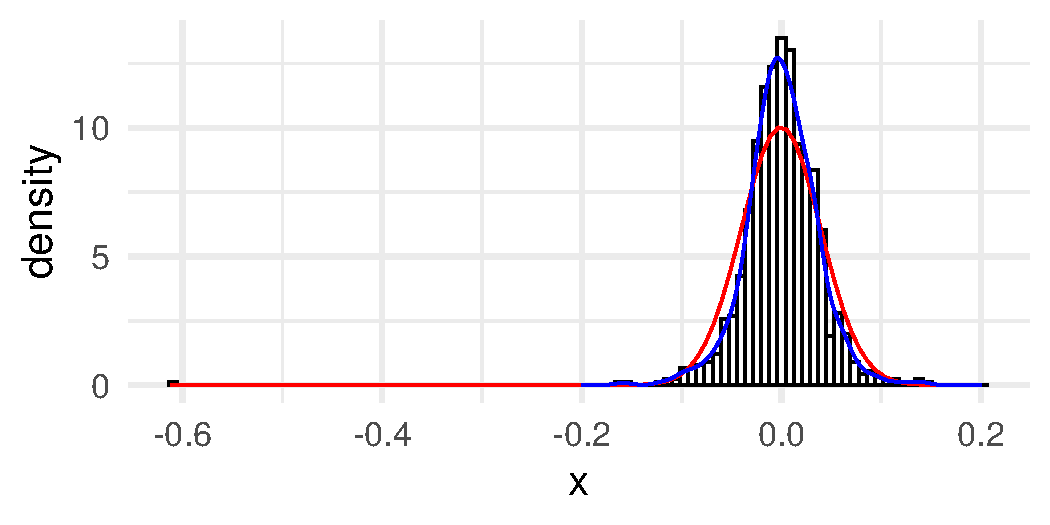
\includegraphics[width=\maxwidth]{figure/unnamed-chunk-25-1} 

\end{knitrout}
